\documentclass[12pt]{article}  
\usepackage{ctex}
\usepackage[“兔”飞猛进]{easymcm}  
\problem{收敛的柯西\_XJ}  
%\usepackage{mathptmx}  
\usepackage{mathpazo}  % 这是 COMAP 官方杂志采用的更好看的 Palatino 字体,可替代以上的 mathptmx 宏包

\title{面向(我)对象}  % 标题


\renewcommand{\contest}{面向对象}

% 文档开始
\begin{document}

\begin{abstract}
UP:

专业:数学与应用数学(师范类)


对象:

专业:信息与计算科学

计划做一个\textbf{视频合集},取名为“面向对象”,当然,不是指编程中的那个意思,主要是针对信息与计算科学专业课后可以学习的技能来进行讲述。由于UP自身专业限制,难免有讲的不好的地方,不当之处,还望海涵。

\noindent 我对象\textbf{不喜欢}:
\begin{enumerate}
    \item 追剧
    \item 听歌
    \item 吃零食
    \item 打游戏(如何:某荣耀)
\end{enumerate}

\noindent \textbf{喜欢}:

\begin{enumerate}
    \item 逛B站
    \item 刷视频(只刷B站)
\end{enumerate}

综上所述,此视频将发布在B站。
\end{abstract}

\maketitle  
\tableofcontents  

\section{Ubuntu系统}

\subsection{认识终端(Terminal)}

终端是连接内核与交互界面的这座桥,它允许用户在交互界面上打开一个叫做「Terminal 终端」的应用程序,在其中输入命令,系统会直接给出反馈。

个人理解:

你在终端输入一行命令,终端可能回复你一下。

\noindent 比如:

\begin{enumerate}
    \item 你输入的命令有误,终端就会给你报错。

    \item 输入 touch a\(.\) txt 
    。在当前目录下就会新建a\(.\) txt文档,但是终端不会告诉你“已成功创建a\(.\)txt ”
\end{enumerate}

\subsubsection{打开终端的方式}

方式一:
\begin{verbatim}
    Ctrl + Alt + T
\end{verbatim}

方式二:

鼠标右键,选择  ``open in terminal"

\newpage
\subsubsection{个人使用的命令}

\begin{table}[h]
\centering
\begin{tabular}{|l|l|}
\hline
\rowcolor[HTML]{FFC702} 
{\color[HTML]{000000} dir} & {\color[HTML]{000000} 列出当前目录下的内容} \\ \hline
ls                         & 列出当前目录下的内容                        \\ \hline
\rowcolor[HTML]{FFC702} 
ls -ah                     & 显示当前路径下的所有内容(包括隐藏文件)              \\ \hline
cd /home                   & 进入“用户列表目录”                       \\ \hline
\rowcolor[HTML]{FFC702} 
cd ..                      & 返回上一级目录                           \\ \hline
cd                         & 进入主目录                             \\ \hline
\rowcolor[HTML]{FFC702} 
pwd                        & 显示工作路径                            \\ \hline
mkdir files                & 在当前路径下新建名为“files”的文件夹             \\ \hline
\rowcolor[HTML]{FFC702} 
rmdir files                & 删除当前路径下名为“files”的文件夹              \\ \hline
touch a.txt                & 新建 a.txt                          \\ \hline
\rowcolor[HTML]{FFC702} 
cat a.txt                  & 输出 a.txt 中的全部内容                   \\ \hline
head a.txt                 & 输出 a.txt 的前10行内容                  \\ \hline
\rowcolor[HTML]{FFC702} 
head -n 5 a.txt            & 输出 a.txt 的前5行内容                   \\ \hline
tail a.txt                 & 输出 a.txt 的最后10行内容(参考head的用法)      \\ \hline
\rowcolor[HTML]{FFC702} 
rm a.txt                   & 删除 a.txt                          \\ \hline
cp a.txt b.txt             & 将 a.txt 的内容复制给 b.txt              \\ \hline
\rowcolor[HTML]{FFC702} 
chmod +x script            & 使script文件可由用户执行                   \\ \hline
\end{tabular}
\end{table}

\textbf{小技巧:}使用方向键(向上和向下),可以浏览命令行使用历史;Ctrl\(+\)c可以取消终端的命令行运行(比如:在终端下载软件时,用Ctrl\(+\)c取消下载)。

\textbf{补充说明:}这里只展示我使用的命令,日后有需要,请百度或者谷歌。

\subsubsection{如何批量创建文件}



\noindent 新建copy.sh文件:
shell脚本
\begin{verbatim}
#!/bin/bash
int=1
while(( $int<=5 ))
do
    cp main.c main${int}.c
    let "int++"
done
\end{verbatim}

\noindent 使用ls查看文件是否可执行(是否为绿色),若不是,使用chmod~ \(+\)x ~copy.sh

\noindent 最后,使用下面的命令运行脚本即可:
\begin{verbatim}
./copy.sh
\end{verbatim}


\subsection{换源}

\href{https://blog.csdn.net/qq_40520596/article/details/110194439}{参考网址(超链接)}

\subsubsection{什么是换源?好处?}
源是 Linux 系统中的一个文件,可以说是 Linux 的灵魂,一个 Linux 配置的源文件决定了 Linux 系统可以获取哪些资源,获取哪些文件,源文件损坏意味着 Linux 系统无法下载 / 更新等。

国外的系统,类似于Ubuntu / Kali / Parrot 这一类系统,默认集成的源是国外的源,使用国外的源下载 / 更新十分缓慢,并且由于速度慢,可能会导致下载错误,中途停止等状况发生,所以国内的源还是十分重要的。
\subsubsection{源文件配置在哪里}
\begin{verbatim}
    /etc/apt/sources.list
\end{verbatim}

\subsubsection{如何换源?}

第一步,“Ctrl + Alt + T”打开终端

第二步,输入命令:sudo su

第三步,输入命令:vim /etc/apt/sources.list

第四步,替换里面的内容(复制镜像网址里面的源文件,然后替换sources.list文件中的内容)

第五步,输入命令:apt-get update

第六步,输入命令:apt-get upgrade

第七步,输入命令:exit


去镜像网址复制源文件,不要用CSDN里面给出的或者其他博主给出的源文件。这里有镜像网址:

\href{https://mirrors.tuna.tsinghua.edu.cn/help/ubuntu/}{https://mirrors.tuna.tsinghua.edu.cn/help/ubuntu/}

\subsection{vim}

\subsubsection{vim是什么?}
从浅层意义上来讲,这就是个编辑器。和你曾经使用过的VScode类似,可以自己配置环境,有代码颜色高亮,含有众多的快捷键等。
\subsubsection{安装vim}
\begin{verbatim}
    sudo apt install vim
\end{verbatim}


\subsubsection{vim的最基本使用方法}
vim共有三种模式(命令模式,写入模式,底线命令模式)。就像迪迦奥特曼一样,具有三种形态:复合型、空中型和强力型。


\noindent \textbf{个人常用的快捷键:}

命令模式下移动光标:

h(左移一单位)

j(下移一单位)

k(上移一单位)

l(右移一单位)

5h(左移5个单位)

即:h~j~k~l的前面可以加上相应的数字,以便于提高光标移动的效率。

\begin{figure}[hbt!]
    \centering
    
\includegraphics[width=0.5\textwidth]{img/j.png}
    \caption{``J"形俄罗斯方块}
\end{figure}

gg(光标移动到首行)

shift + g(光标移动到最后一行)

从命令模式进入写入模式:

i(insert)

shift + i

shift + a

退出写入模式:

Esc

此时进入命令模式

保存文档并退出vim:

在命令模式下,按“:”(英文状态),进入底线命令模式,输入“wq”,然后按“Enter”即可退出。

\begin{verbatim}
w for write

q for quit
    
\end{verbatim}






\noindent \textbf{修改相关的配置(参考如下教程,留作课后作业):}
\begin{enumerate}
    \item 配置.vimrc 文件

使用快捷键:“Ctrl + Alt + T”,打开终端,使用vim .vimrc 命令。

\begin{figure}[h]
    \centering
    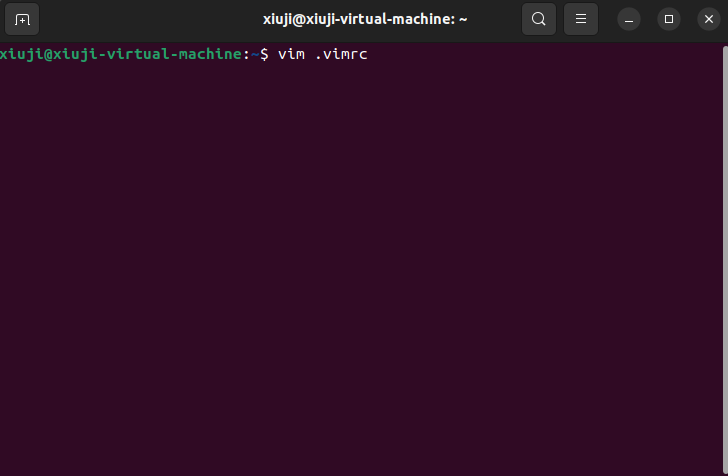
\includegraphics[width=0.7\textwidth]{img/.vimrc.png}
    \caption{进入.vimrc文件}
\end{figure}

将下面的代码粘贴进.vimrc里面可以调节tab键的空格数目(4个)

\begin{verbatim}
" add tab space
set ts=4
set softtabstop=4
set shiftwidth=4
set expandtab
set autoindent
\end{verbatim}

解释一下:

ts 是tabstop的缩写,设TAB宽度为4个空格。

softtabstop 表示在编辑模式的时候按退格键的时候退回缩进的长度,当使用 expandtab 时特别有用。

shiftwidth 表示每一级缩进的长度,一般设置成跟 softtabstop 一样。

expandtab表示缩进用空格来表示,noexpandtab 则是用制表符表示一个缩进。

autoindent自动缩进    

\begin{figure}[h]
    \centering
    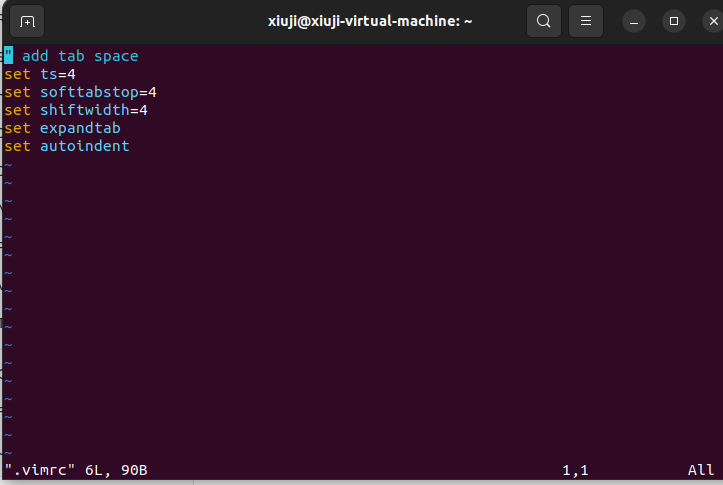
\includegraphics[width=0.7\textwidth]{img/fixvim.png}
    \caption{把相应的内容写进去}
\end{figure}
\newpage
\item 把Caps Lock键映射成Esc键:
\begin{verbatim}
sudo apt install gnome-tweaks

gnome-tweaks
\end{verbatim}

\begin{figure}[hbt!]
    \centering
    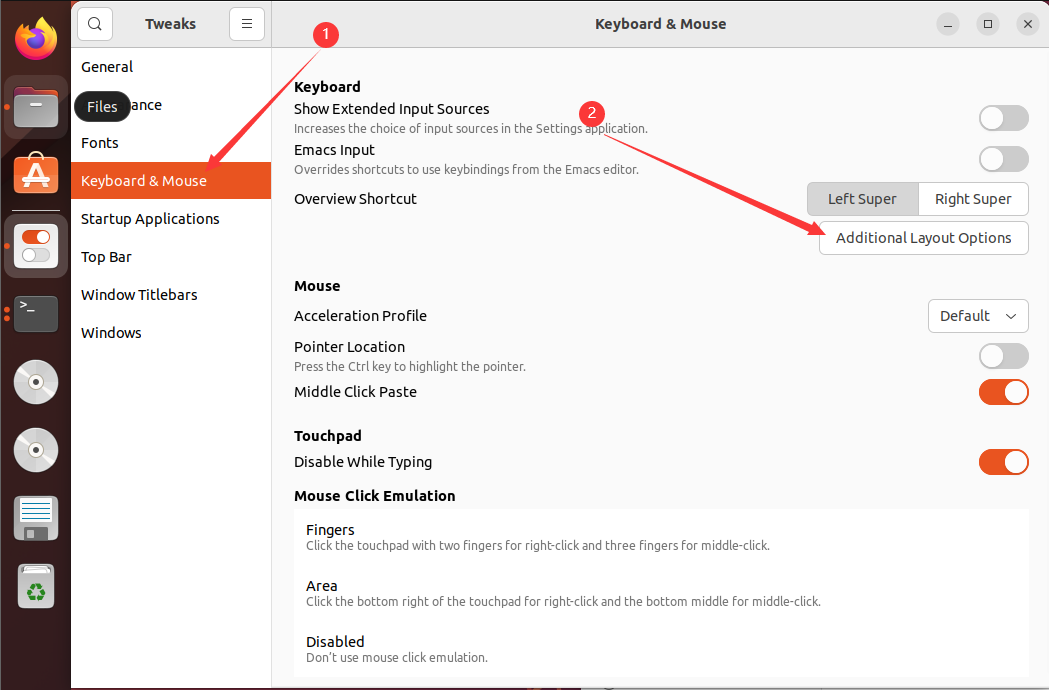
\includegraphics[width=0.9\textwidth]{img/one.png}
    \caption{第一步}
\end{figure}

\begin{figure}[hbt!]
    \centering
    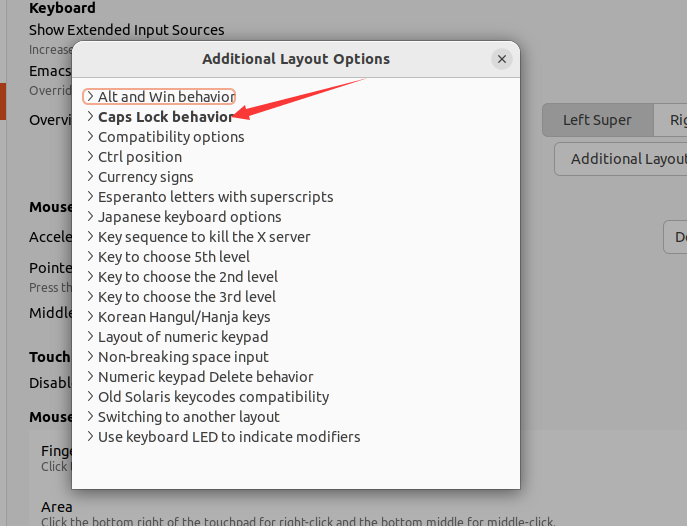
\includegraphics[width=0.8\textwidth]{img/two.png}
    \caption{第二步}
\end{figure}

\begin{figure}[hbt!]
    \centering
    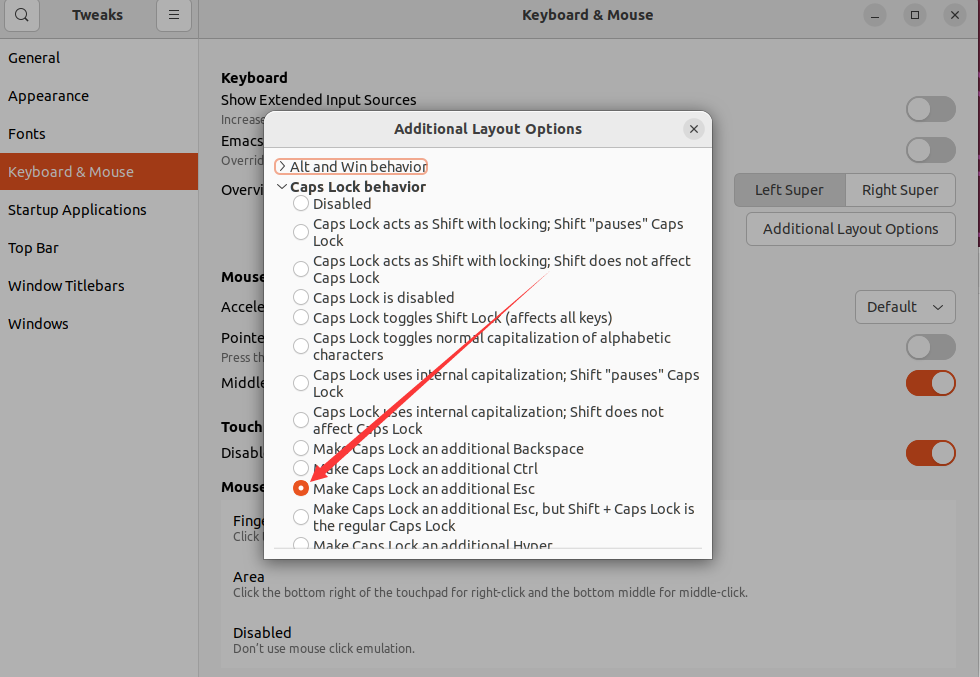
\includegraphics[width=0.8\textwidth]{img/three.png}
    \caption{第三步}
\end{figure}
\newpage

\item 举个例子

\begin{verbatim}
vim hello.c
\end{verbatim}

此时在当前路径下创建hello.c文件并打开hello.c文件(进入“命令模式”)。

若当前路径已经有hello.c文件,则直接打开hello.c文件(进入“命令模式”)。

接着,按“i”进入“写入模式”

此时,可以写:
\begin{verbatim}
#include <stdio.h>
int main()
{
    printf("hello world!\n");
    return 0;
}
\end{verbatim}

写完后,按“Esc”键退出“写入模式”;(但是我们已经把Caps Lock键映射成Esc键,所以,此时也可以直接按“Caps Lock”键退出“写入模式”)

此时,已经进入了“命令模式”,按英文状态下“:”(冒号)键,进入“底线命令模式”,输入wq,然后回车,即可退出vim。

w for write(写入)

q for quit(退出)


较详细使用方法参考:

\href{https://www.runoob.com/linux/linux-vim.html}{https://www.runoob.com/linux/linux-vim.html}

\end{enumerate}


\subsection{安装软件}

说明一下,apt 是Ubuntu系统的包管理器

\subsubsection{命令行安装软件}
比如在上文中,有安装vim的操作:

\begin{verbatim}
    sudo apt install vim
\end{verbatim}

\newpage
\subsubsection{软件商店直接安装}

\begin{figure}[hbt!]
    \centering
    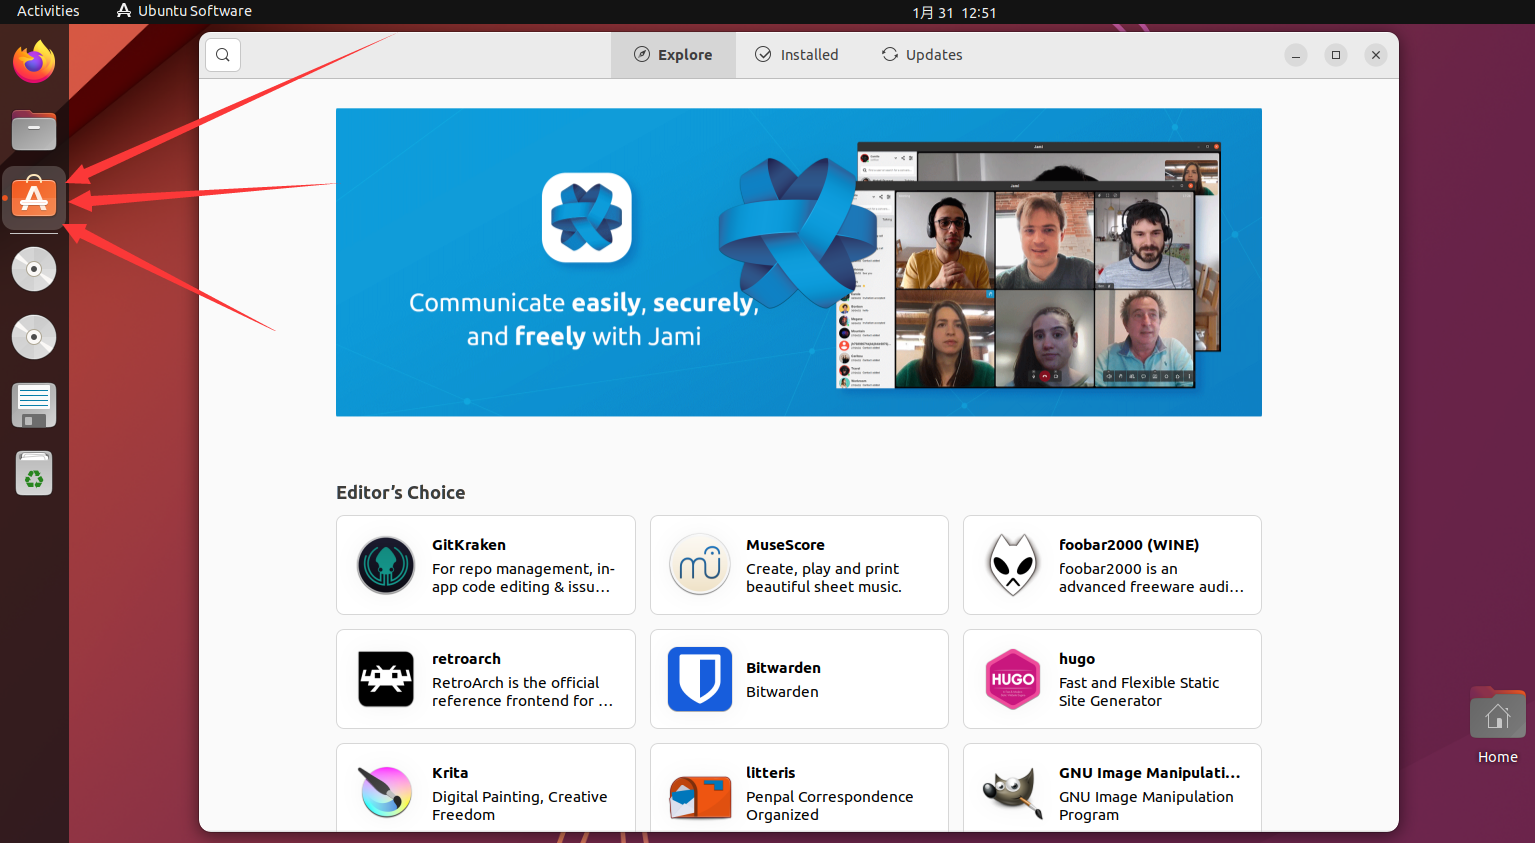
\includegraphics[width=0.7\textwidth]{img/software.png}
    \caption{Ubuntu software}
\end{figure}

\subsubsection{网上下载.deb安装包结合相关命令}

这里以安装QQ为例子

1.官网下载Linux版本的QQ(.deb)安装包

\href{https://im.qq.com/linuxqq/index.shtml}{https://im.qq.com/linuxqq/index.shtml}

\begin{figure}[hbt!]
    \centering
    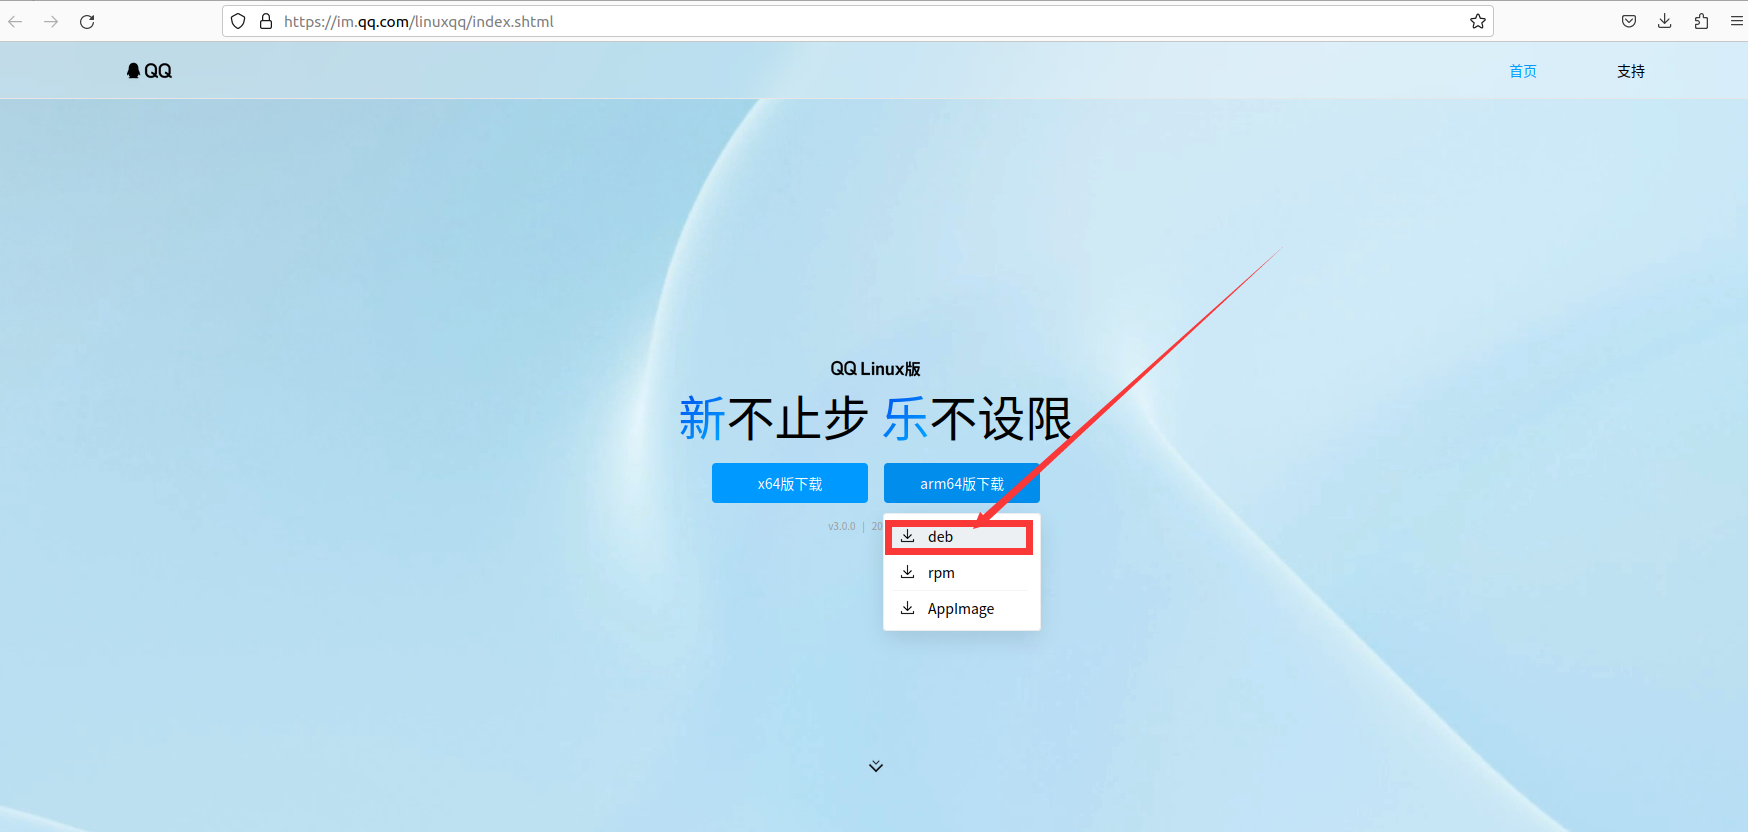
\includegraphics[width=0.82\textwidth]{img/qqforlinux.png}
    \caption{qqforlinux}
\end{figure}

2.打开终端,切换目录到安装包所在位置

3.输入命令:sudo dpkg -i linuxqqbalabalabala.deb

如图\ref{installforqq}所示

\begin{figure}[hbt!]
    \centering
    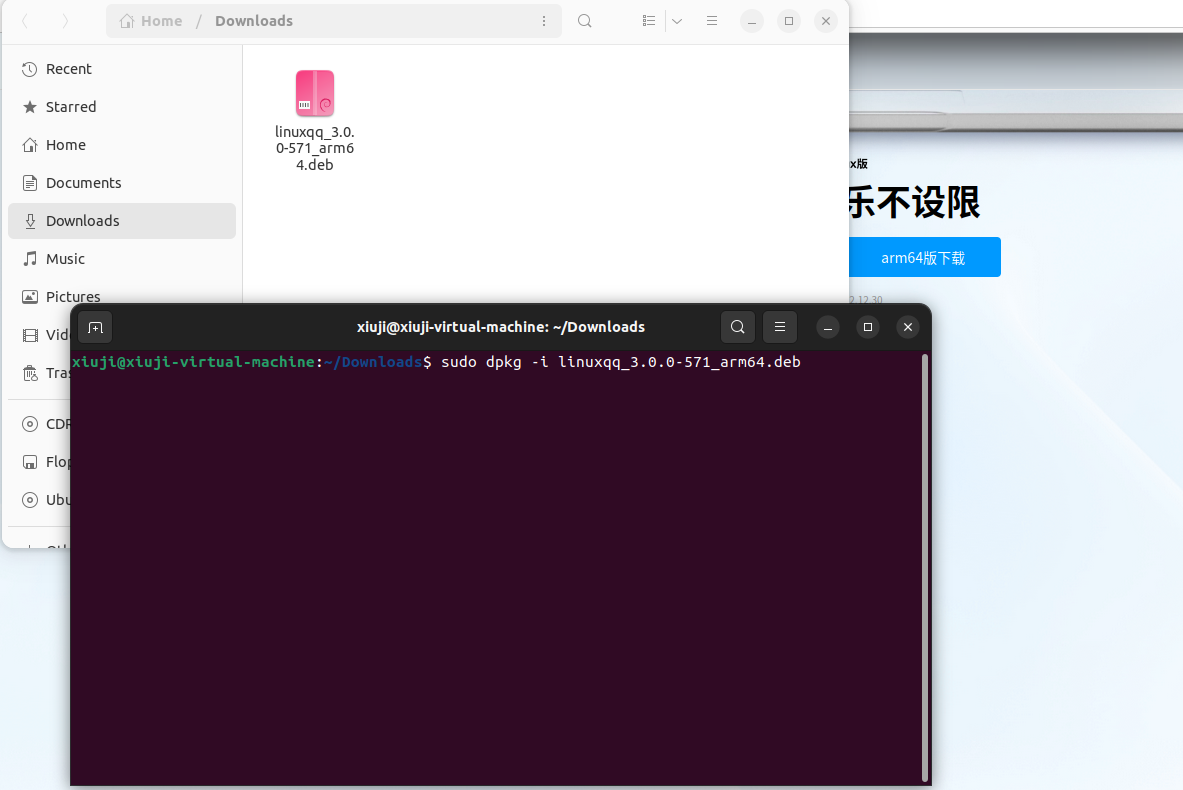
\includegraphics[width=0.9\textwidth]{img/installforqq.png}
    \caption{installqq}
    \label{installforqq}
\end{figure}




\newpage
\subsection{在终端运行python}

\begin{verbatim}
    python3 --version   可以查看python版本

    python3 hello.py     运行hello.py文件

    sudo apt install python3-numpy  安装numpy(第三方库)

    pip list        查看已安装的库
\end{verbatim}


\subsection{卸载}

参考:
\href{https://zhuanlan.zhihu.com/p/339632982}{https://zhuanlan.zhihu.com/p/339632982}

\subsubsection{配置pycharm}

在设置界面......

\subsection{在终端运行Java}

\href{https://linux.cn/article-13790-1.html}{https://linux.cn/article-13790-1.html}

\subsection{C语言文件的编译、连接}

\subsubsection{gcc安装}

\begin{verbatim}
    sudo apt install gcc
\end{verbatim}

\subsubsection{举个例子}

main.c文件内容如下:

\begin{lstlisting}
#include <stdio.h>
int main()
{
    printf("hello world!\n");
    return 0;
}
\end{lstlisting}

在终端输入以下的命令方可输出“hello world!”
\begin{verbatim}
    gcc main.c -o myproject

    ./myproject
\end{verbatim}



\subsection{报错了?如何百度(or~ 必应 ~or~ 谷歌)}
直接复制报错的信息,粘贴至浏览器去搜索



\section{Windows系统}

\subsection{cmd(命令提示符)}
打开方式:
\begin{verbatim}
    win + R 打开“运行”,输入cmd,回车
\end{verbatim}

具体可以参考下面的图片
\begin{figure}[hbt!]
    \centering
    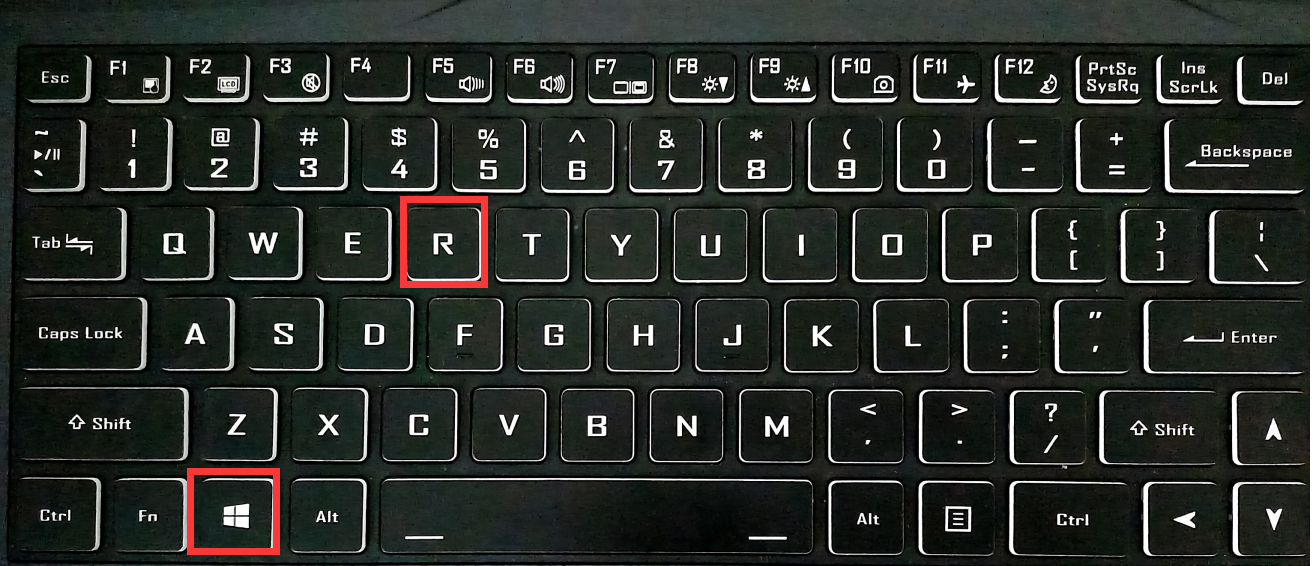
\includegraphics[width = 0.5\textwidth]{img/winjiar.png}
    \caption{win + R}
\end{figure}

\begin{figure}[hbt!]
    \centering
    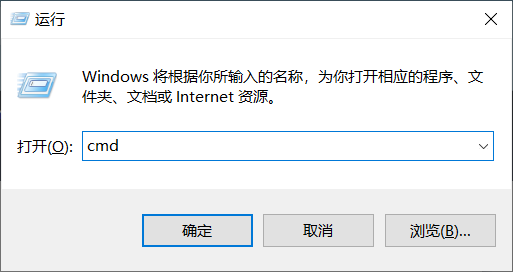
\includegraphics[width = 0.5\textwidth]{img/cmd.png}
    \caption{输入cmd}
\end{figure}
\newpage


以管理员身份打开:

\begin{figure}[hbt!]
    \centering
    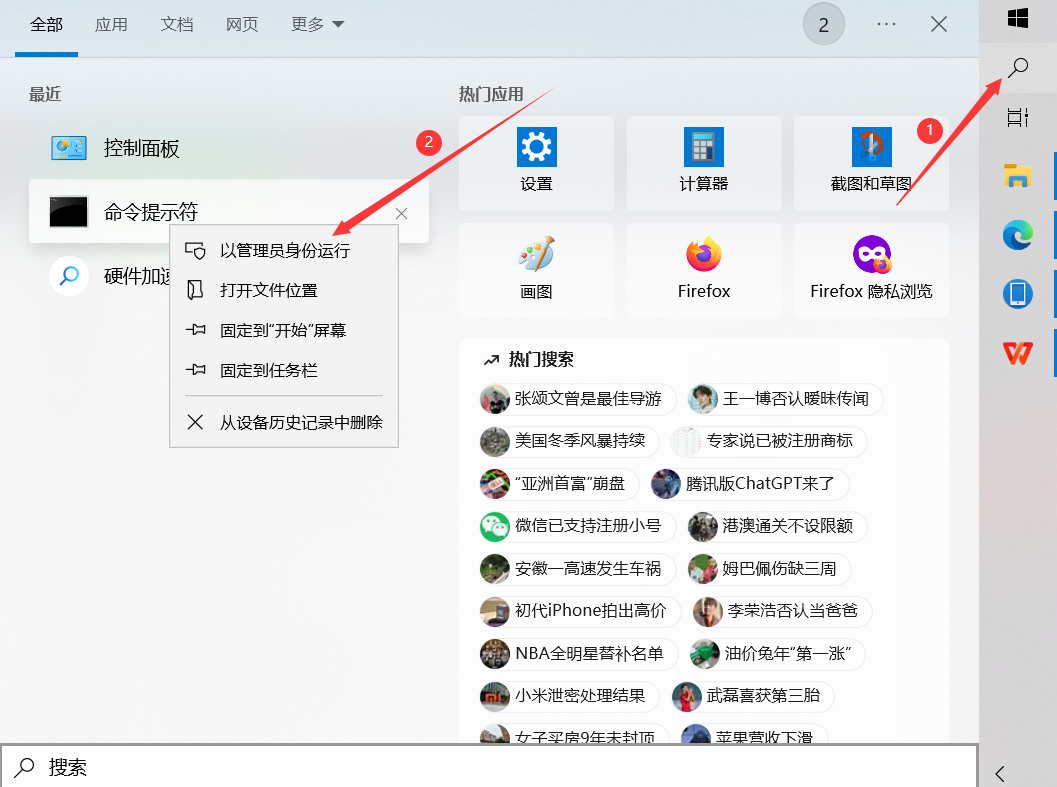
\includegraphics[width=0.5\textwidth]{img/guanliyuanshenfen.png}
    \caption{以管理员身份打开}
\end{figure}


\subsubsection{个人使用的命令}
\begin{verbatim}
    cd
    dir
    这两个命令的使用方法和在Linux中一样
\end{verbatim}

\subsubsection{python文件转为.exe文件}

\subsection{Powershell打开方式}

\subsection{安装软件}

\subsection{卸载软件}

\section{Git与GitHub}

参考地址:
\href{https://www.liaoxuefeng.com/wiki/896043488029600}{https://www.liaoxuefeng.com/wiki/896043488029600}

\subsection{Git简介}
\href{https://www.liaoxuefeng.com/wiki/896043488029600/896067008724000}{https://www.liaoxuefeng.com/wiki/896043488029600/896067008724000}

\subsubsection{Git诞生}
\href{https://www.liaoxuefeng.com/wiki/896043488029600/896202815778784}{https://www.liaoxuefeng.com/wiki/896043488029600/896202815778784}
\subsubsection{集中式VS分布式}
\href{https://www.liaoxuefeng.com/wiki/896043488029600/896202780297248}{https://www.liaoxuefeng.com/wiki/896043488029600/896202780297248}
\subsection{安装Git}
\href{https://www.liaoxuefeng.com/wiki/896043488029600/896067074338496}{https://www.liaoxuefeng.com/wiki/896043488029600/896067074338496}
\subsection{创建版本库}
\href{https://www.liaoxuefeng.com/wiki/896043488029600/896827951938304}{https://www.liaoxuefeng.com/wiki/896043488029600/896827951938304}
\subsection{版本回退}
\href{https://www.liaoxuefeng.com/wiki/896043488029600/897013573512192}{https://www.liaoxuefeng.com/wiki/896043488029600/897013573512192}
\subsection{工作区和暂存区}
\href{https://www.liaoxuefeng.com/wiki/896043488029600/897271968352576}{https://www.liaoxuefeng.com/wiki/896043488029600/897271968352576}
\subsection{管理修改}
\href{https://www.liaoxuefeng.com/wiki/896043488029600/897884457270432}{https://www.liaoxuefeng.com/wiki/896043488029600/897884457270432}
\subsection{撤销修改}
\href{https://www.liaoxuefeng.com/wiki/896043488029600/897889638509536}{https://www.liaoxuefeng.com/wiki/896043488029600/897889638509536}
\subsection{删除文件}
\href{https://www.liaoxuefeng.com/wiki/896043488029600/900002180232448}{https://www.liaoxuefeng.com/wiki/896043488029600/900002180232448}
\subsection{远程仓库}
\href{https://www.liaoxuefeng.com/wiki/896043488029600/896954117292416}{https://www.liaoxuefeng.com/wiki/896043488029600/896954117292416}
\subsubsection{添加远程库}
\href{https://www.liaoxuefeng.com/wiki/896043488029600/898732864121440}{https://www.liaoxuefeng.com/wiki/896043488029600/898732864121440}
\subsubsection{从远程库克隆}
\href{https://www.liaoxuefeng.com/wiki/896043488029600/898732792973664}{https://www.liaoxuefeng.com/wiki/896043488029600/898732792973664}
\subsection{分支管理}
自学

\href{https://www.liaoxuefeng.com/wiki/896043488029600/896954848507552}{https://www.liaoxuefeng.com/wiki/896043488029600/896954848507552}

\subsection{Git关联Gitee}

\section{免费下载文献}

\begin{enumerate}
    \item 知网

“校外访问”即可

    \item 维普
    
    \href{http://www.cqvip.com/}{http://www.cqvip.com/}
    \item google学术

    \href{https://scholar.google.com/}{https://scholar.google.com/}

    \href{https://so.hiqq.com.cn/}{https://so.hiqq.com.cn/}

    \href{https://scholar.lanfanshu.cn/}{https://scholar.lanfanshu.cn/}
\end{enumerate}
\end{document}